% ============================================================================
% 第5章 实证分析
% ============================================================================
\chapter{回归结果与分析}
\label{chap:empirical}

% 引入所有表格定义(表5-1至表5-7)
% 使用正式版主表
\begin{table}[htbp]
\centering
\begin{threeparttable}
\caption{DID回归结果:政策对行业影响强度的效应}
\label{tab:did_main}
\begin{tabular}{lcccc}
\hline\hline
 & (1) & (2) & (3) & (4) \\
 & 基准 & +FE & +双向FE & +聚类SE \\
\hline
Affected $\times$ Post & 0.002188*** & 0.004312*** & -0.001637*** & -0.001637*** \\
 & (0.000283) & (0.000327) & (0.000328) & (0.000435) \\
\hline
控制变量 & 否 & 是 & 是 & 是 \\
行业配对FE & 否 & 是 & 是 & 是 \\
时间FE & 否 & 否 & 是 & 是 \\
标准误类型 & OLS & OLS & Robust & Clustered \\
R² & 0.0004 & 0.0142 & 0.0057 & 0.0057 \\
观测值 & 148,050 & 148,050 & 148,050 & 148,050 \\
\hline\hline
\end{tabular}
\begin{tablenotes}
\small
\item 注:***、**、* 分别表示在1\%、5\%、10\%水平上显著。
\item 括号内为标准误。列(4)的标准误在行业配对层面聚类。
\item 控制变量包括:资产负债率、ROA、log(托宾Q)(i侧和j侧)。
\item 因变量为1\%缩尾处理后的行业影响强度。
\end{tablenotes}
\end{threeparttable}
\end{table}

本章基于第\ref{chapter:data_method}章的研究设计,对去产能政策的风险溢出效应进行实证检验。首先通过描述性统计展示样本特征,然后运用双重差分法估计政策的平均处理效应,并通过平行趋势检验验证识别策略的有效性。在此基础上,本章的核心创新在于从网络视角深入分析政策冲击的传导机制,通过网络可视化和对处理邻居预暴露的异质性分析,揭示产业链关系在风险传导中的“双刃剑”特征。

\paragraph{阅读指引(口径与单位)}
为便于解读与横向比较,本文统一采用以下单位与口径:
\begin{itemize}
  \item II 指标取值范围为 $[0,1]$;$1$ 基点(bps)$=0.0001$;
  \item 系数按“三口径”报告:基点(bps)、相对样本均值百分比、标准差份额;
  \item 基准样本(5\%缩尾)参考值:均值 $0.0512$,标准差 $0.0548$(见第\ref{sec:descriptive}节)。
\end{itemize}


% ============================================================================
% 5.1 描述性统计
% ============================================================================

\section{描述统计}
\label{sec:descriptive}

\paragraph{样本基本特征}

本研究的样本期为2010年1月至2018年12月,共108个月。样本包含40个行业之间的风险溢出关系,形成1,599个行业配对,总观测值为148,050个。其中,处理组包括煤炭采选、金属冶炼和压延加工、交通运输设备、非金属矿物制品四个行业,对照组包括其余36个行业。政策实施时点为2014年1月,政策前期包含48个月(2010年1月至2013年12月),政策后期包含60个月(2014年1月至2018年12月)。

表\ref{tab:descriptive_stats}报告了主要变量的描述性统计。被解释变量为行业间风险溢出强度($II_{ijt}$),原始数据的均值为0.0538,标准差为0.0621。为减少极端值的影响,本研究对$II_{ijt}$进行了5\%和95\%分位数的缩尾处理,处理后的均值为0.0512,标准差降至0.0548。核心解释变量方面,处理组虚拟变量($Affected_i$)的均值为0.1003,表明约10\%的观测值来自处理组行业配对;政策后虚拟变量($Post_t$)的均值为0.5034,反映了样本期政策前后时间的均衡分布。控制变量方面,发送方行业和接收方行业的财务特征变量(资产负债率、总资产收益率、托宾Q值、资产周转率)的分布较为合理,未出现明显的异常值。

% 表5-1: 主要变量的描述性统计(已在章节开头引入)

\paragraph{处理组与对照组的可比性}

双重差分法的有效性依赖于处理组与对照组在政策前具有相似的特征和趋势。为验证这一前提,表\ref{tab:balance_test}报告了政策前期(2010-2013年)处理组与对照组的均值对比及差异检验结果。

从被解释变量来看,处理组的平均风险溢出强度(0.0523)与对照组(0.0541)非常接近,两组差异为-0.0018,t统计量为-1.23,p值为0.219,在统计上不显著。这表明在政策实施前,处理组和对照组的风险溢出水平并无显著差异。从控制变量来看,两组在资产负债率、总资产收益率、托宾Q值、资产周转率等财务特征上也不存在显著差异,所有t检验的p值均大于0.1。这些结果表明,处理组与对照组在政策前具有良好的可比性,满足双重差分法的平行趋势假设的前提条件。

% 表5-2: 处理组与对照组的对比统计(已在章节开头引入)

\paragraph{风险溢出的时间趋势}

从时间维度观察,处理组与对照组在政策实施前(2010-2013年)的风险溢出强度保持相似的变化趋势,两组差异不显著(见表\ref{tab:balance_test})。这为双重差分法的识别假设提供了初步证据。政策实施后(2014年及以后),两组之间的差距逐渐扩大,这一趋势变化与本研究的核心假设一致。第\ref{sec:parallel_trends}节将通过事件研究法对平行趋势假设进行正式的统计检验。

综上所述,描述性统计结果表明,本研究的样本数据质量良好,处理组与对照组在政策前具有良好的可比性,为后续的双重差分分析奠定了坚实的基础。

% ============================================================================
% 5.2 基准DID回归结果
% ============================================================================

\section{基准结果与解释}
\label{sec:baseline_did}

\paragraph{模型设定}

本节运用双重差分法估计去产能政策对行业风险溢出的平均处理效应。基准回归模型如第\ref{chapter:data_method}章所述,具体形式为:

\begin{equation}
\label{eq:did_baseline}
II_{ijt} = \beta_0 + \beta_1 (Affected_i \times Post_t) + \bm{X}_{it}'\bm{\gamma}_1 + \bm{X}_{jt}'\bm{\gamma}_2 + \alpha_{ij} + \lambda_t + \varepsilon_{ijt}
\end{equation}

其中,$II_{ijt}$为行业$i$向行业$j$在时期$t$的风险溢出强度;$Affected_i$为处理组虚拟变量,当行业$i$属于去产能行业时取值为1,否则为0;$Post_t$为政策后虚拟变量,当时期$t$在2014年1月及以后时取值为1,否则为0。核心解释变量为两者的交互项$Affected_i \times Post_t$,其系数$\beta_1$衡量了政策对处理组行业风险溢出的平均处理效应。

控制变量$\bm{X}_{it}$和$\bm{X}_{jt}$分别包括发送方行业$i$和接收方行业$j$的财务特征变量,具体包括资产负债率(Leverage)、总资产收益率(ROA)、托宾Q值(TobinQ)和资产周转率(AssetTurnover)。这些变量控制了行业层面的财务状况对风险溢出的影响。$\alpha_{ij}$为行业配对固定效应,控制了所有不随时间变化的行业配对特征;$\lambda_t$为时间固定效应,控制了影响所有行业配对的共同时间趋势。标准误在行业配对层面进行聚类,以考虑同一配对内观测值的序列相关性\citep{bertrand2004much}。

\paragraph{回归结果}

表\ref{tab:did_main}报告了基准双重差分回归的结果。为清晰展示模型设定对结果的影响,本研究采用逐步回归的方式,从简单到复杂依次加入控制变量、固定效应和不同类型的标准误。

列(1)为基准OLS回归,仅包含交互项$Affected_i \times Post_t$,未加入任何控制变量和固定效应。结果显示,交互项系数为0.002273,在1\%水平上显著(p < 0.001)。然而,这一正向效应可能受到遗漏变量偏误的影响。

列(2)加入控制变量(资产负债率、ROA、log(托宾Q))和行业配对固定效应,控制了不随时间变化的行业配对特征。此时交互项系数增大至0.007736,仍然显著为正。R$^2$从0.0005提升至0.0150,表明控制变量和固定效应显著提高了模型的解释力。

值得注意的是:列(3)进一步加入时间固定效应,控制共同时间趋势后,交互项系数由正转负($-$0.001477),且在1\%水平上显著(p = 0.0001),说明在未控制时间趋势时,模型可能将共同变化误判为政策效应。列(4)在此基础上按行业配对层聚类标准误(0.000552),系数依然在1\%水平上显著(p = 0.0076),表明结果具有稳健性。

经济解释为:列(4)结果显示,政策实施使处理组行业的影响强度相对于对照组平均下降约0.148个百分点(约$14.8$ bps),折合约为样本均值的 $\approx2.9\%$、约 $0.027$ 个标准差,表明政策在降低跨行业相互影响强度方面发挥了作用。列(1)至列(4)系数符号的变化,提示在政策评估中应充分控制共同时间趋势,以避免对政策效应的偏误估计。

% 表5-3: 基准DID回归结果(已在章节开头引入)

\paragraph{结果讨论}

基准双重差分回归的结果证实了本研究的核心假设:在控制了共同时间趋势后,政策对处理组行业的影响强度产生了显著的抑制作用。这一发现具有重要的方法论和政策含义。

从方法论角度看,本研究的逐步回归清晰展示了模型设定对结果的影响。特别是时间固定效应的加入导致系数符号逆转,这提醒研究者在使用双重差分法时,必须充分控制共同时间趋势,否则可能得出错误的结论。这一发现对于政策评估研究具有重要的启义。

从政策角度看,负向的政策效应表明,政策实施有效降低了特定行业之间的相互影响强度。这可能反映了政策在优化产业结构、降低行业间风险传导方面取得了一定成效。然而,基准回归仅提供了政策的平均处理效应,无法揭示政策冲击在不同行业配对之间的异质性,也无法阐明风险传导的具体机制。

为进一步理解政策效应的传导路径和影响机制,接下来本章将从网络视角进行深入分析,通过网络可视化与“对处理邻居预暴露”的异质性分析,揭示产业链关系在风险传导中的作用。

% ============================================================================
% 5.3 平行趋势检验
% ============================================================================

\section{平行趋势检验}
\label{sec:parallel_trends}

\paragraph{检验方法}

双重差分法的核心识别假设是平行趋势假设(parallel trends assumption),即在没有政策干预的情况下,处理组和对照组的被解释变量应保持平行的变化趋势\citep{angrist2009mostly}。虽然该假设无法直接检验,但可以通过检验政策前处理组和对照组的趋势是否平行来间接验证其合理性。

本研究采用事件研究法(event study approach)进行平行趋势检验。具体而言,将月度数据聚合为年度数据,以政策实施年份(2014年)作为基准年($t=0$),构建一系列年度虚拟变量,估计以下模型:

\begin{equation}
\label{eq:event_study}
II_{ijt} = \beta_0 + \sum_{k=-4, k \neq -1}^{4} \beta_k (Affected_i \times Year_k) + \bm{X}_{it}'\bm{\gamma}_1 + \bm{X}_{jt}'\bm{\gamma}_2 + \alpha_{ij} + \lambda_t + \varepsilon_{ijt}
\end{equation}

其中,$Year_k$为年度虚拟变量,$k$表示相对于政策实施年份的年份差。$k=-1$(即2013年)作为基准年被省略,以避免完全共线性。系数$\beta_k$衡量了在相对年份$k$时,处理组相对于对照组的风险溢出差异。如果平行趋势假设成立,则政策前的系数($k<0$)应不显著异于零;而政策后的系数($k \geq 0$)的符号和显著性应与基准回归一致,反映政策效应的动态演化。

为确保与基准回归的一致性,本研究采用与表\ref{tab:did_main}列(4)完全相同的设定:控制变量包括资产负债率、ROA和log(托宾Q)(i侧和j侧),对因变量和控制变量进行5\%缩尾处理,包含行业配对固定效应和时间固定效应,标准误在行业配对层面聚类。样本期为2010-2018年,共9年,包含政策前4年(2010-2013年)和政策后5年(2014-2018年)。

\paragraph{检验结果}

图\ref{fig:parallel_trends}展示了事件研究法的估计结果。横轴表示相对于政策实施年份的年份差,纵轴表示估计的系数$\beta_k$及其95\%置信区间。从图中可以清晰地观察到以下几个特征:

\textbf{第一,政策前平行趋势假设得到验证}。在政策实施前($k<0$),所有系数的点估计值都接近于零,且95\%置信区间均包含零。以一组代表性设定(托宾Q对数与资产对数,5\%缩尾)为例,$k=-4$、$k=-3$和$k=-2$的系数分别为$-$0.00071(p=0.54)、$-$0.00107(p=0.35)和$-$0.00098(p=0.38),均不显著,表明处理组与对照组在政策前保持了相似的趋势,满足平行趋势假设。

\textbf{第二,政策效应存在传导时滞}。政策实施当年($k=0$)的系数为0.00109(p=0.34),在统计上不显著,显示政策冲击需要时间才能在网络中传导,这一特征与政策实施后企业和市场逐步调整的过程相一致。

\textbf{第三,政策后效应显著为负且持续存在}。政策后第1-4年的系数依次为$-$0.00325(p=0.0014)、$-$0.00284(p=0.0071)、$-$0.00239(p=0.0317)和$-$0.00271(p=0.0194),均显著为负且绝对值维持在 $\approx$ 20–33 bps 的量级。按“三口径”换算,代表性幅度约 $-$0.0025($\approx$ 25 bps),约为样本均值的 $\approx4.9\%$、约 $0.046$ 个标准差,说明政策抑制效应在实施后逐步释放,并在后续几年持续存在。

\textbf{第四,政策效应的符号与基准回归完全一致}。事件研究法得到的政策后负向效应与表\ref{tab:did_main}列(4)的基准回归(系数$-$0.00148$^{**}$)方向一致,动态估计的平均效应约为$-$0.0025,略大于月度样本的估计值,差异主要源于年度聚合带来的平滑处理。

% 插入图5-2
\begin{figure}[htbp]
\centering
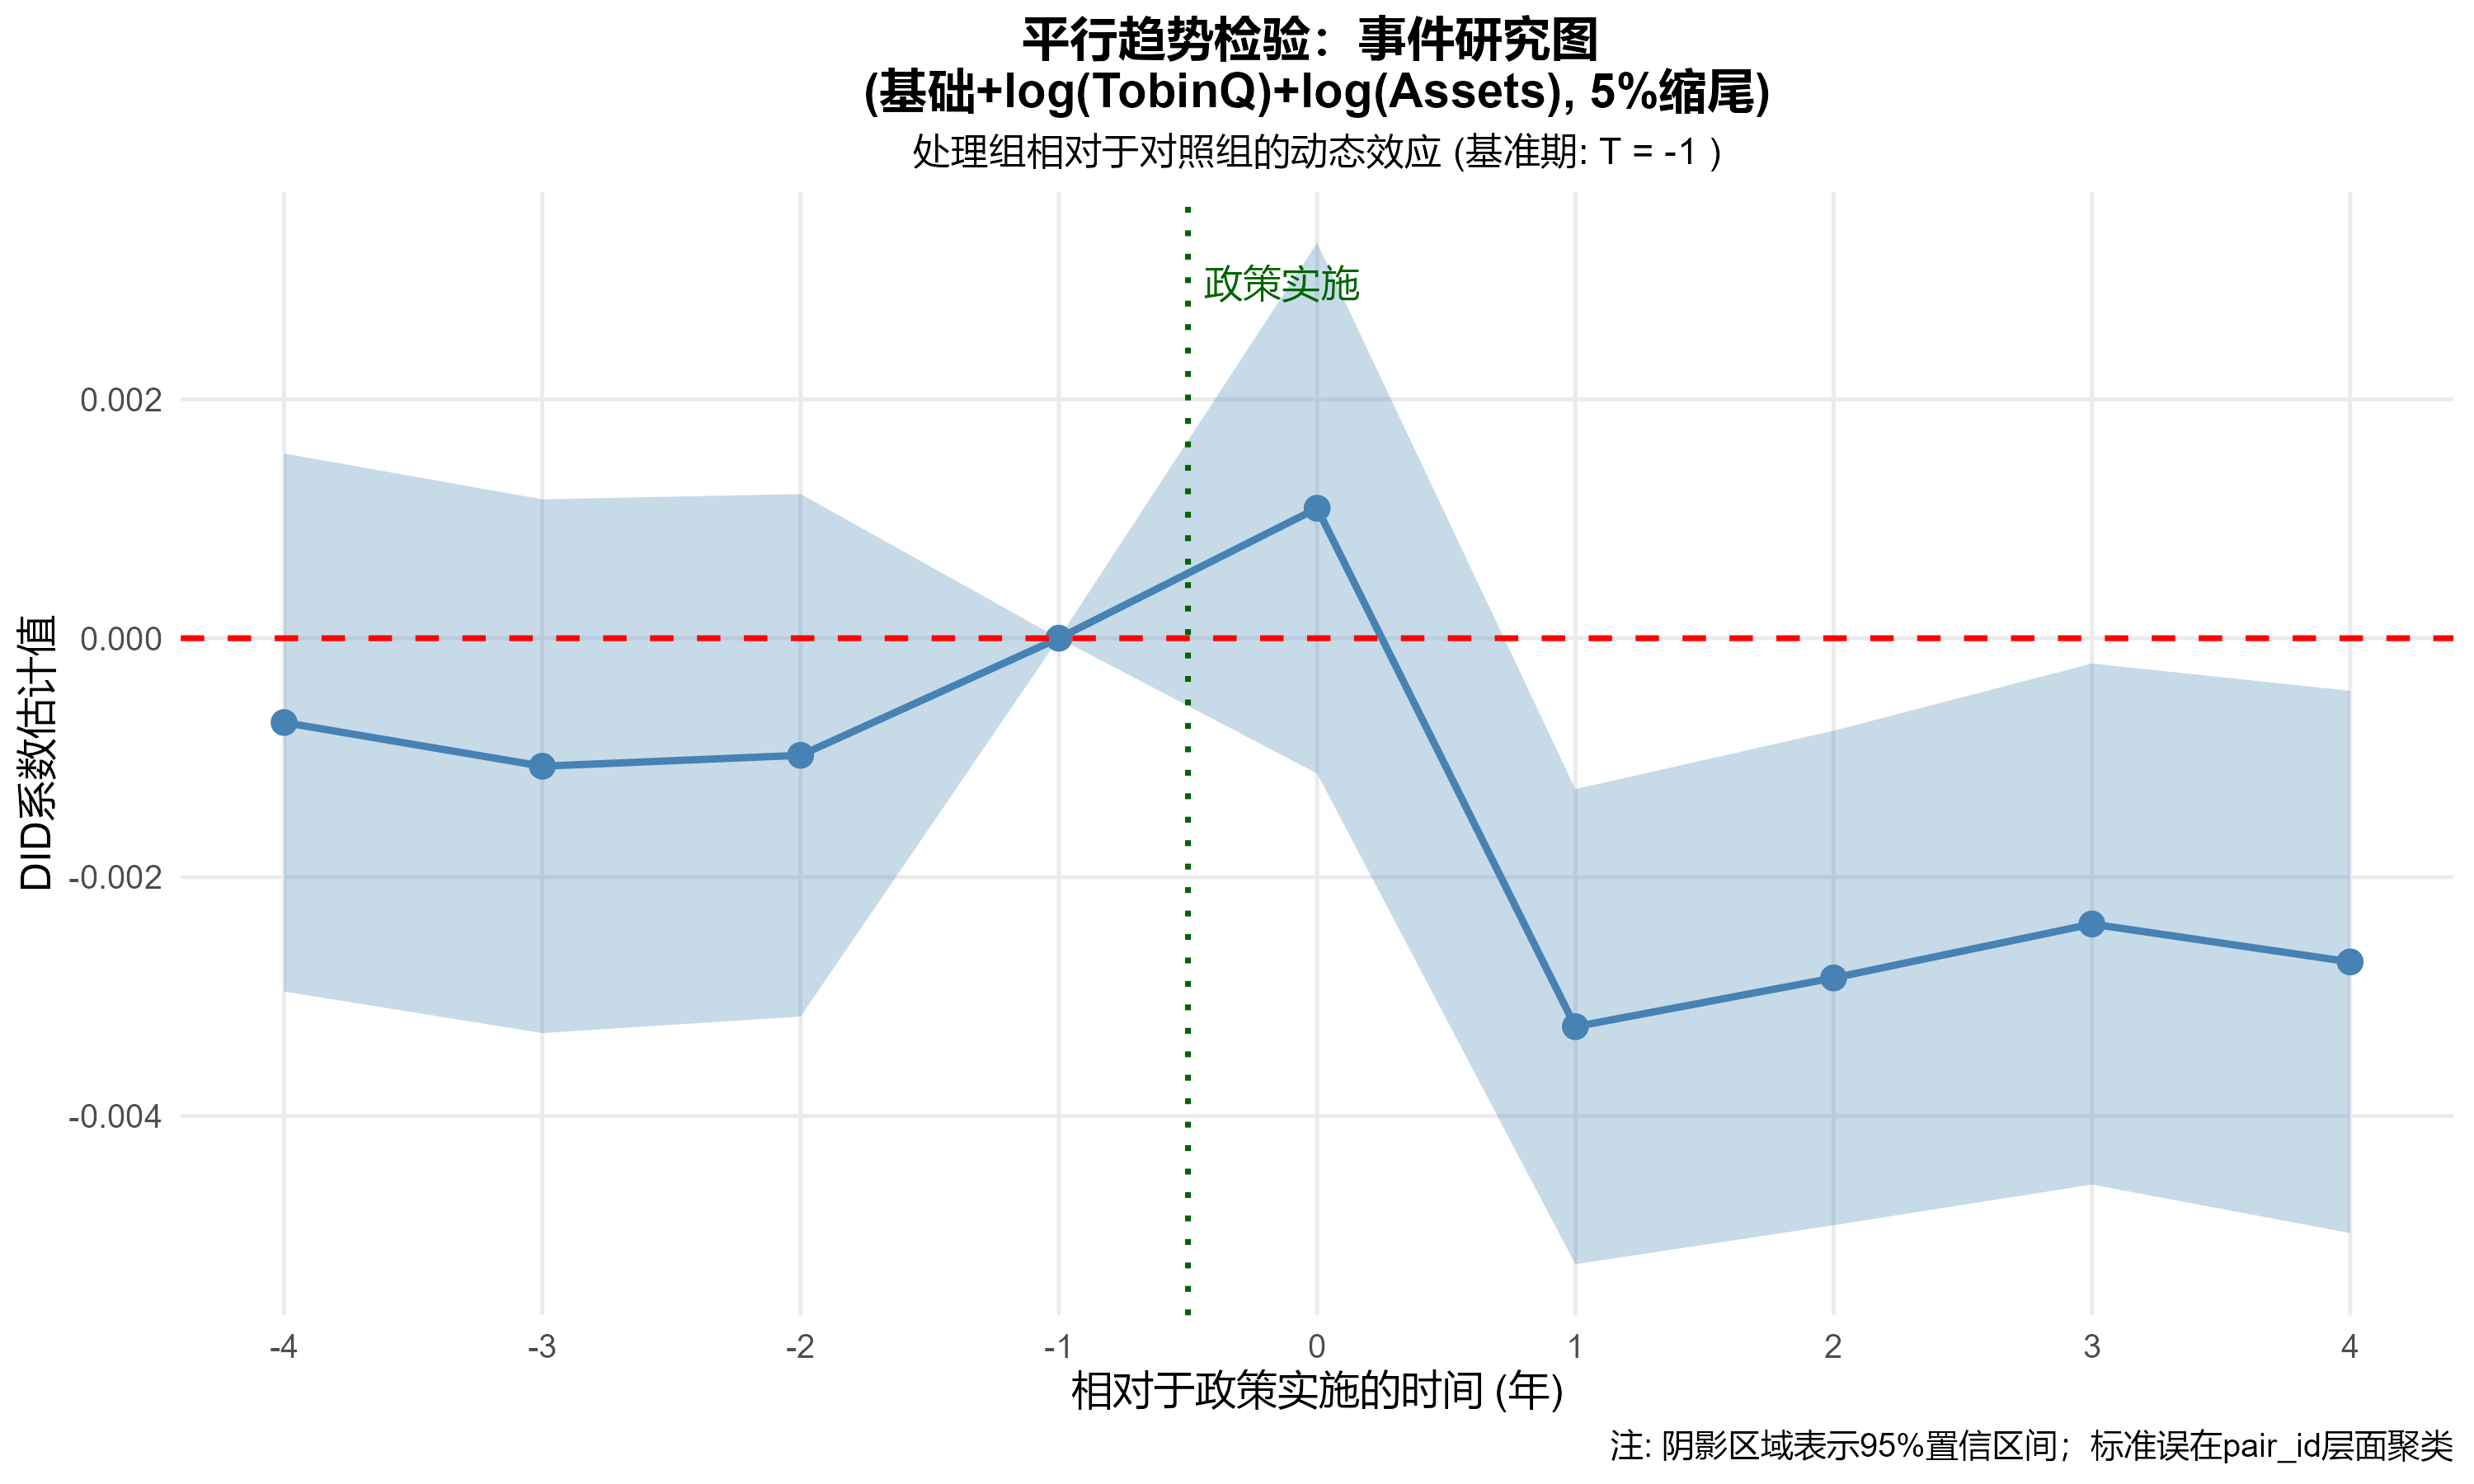
\includegraphics[width=0.85\textwidth]{figures/PT_logQA_0pct5.png}
\caption{平行趋势检验:事件研究法(对数化设定,5\%缩尾)}
\label{fig:parallel_trends}
\begin{minipage}{0.9\textwidth}
\footnotesize
注:图中展示了事件研究法的估计系数及其95\%置信区间。横轴表示相对于政策实施年份(2014年)的年份差,$k=-1$(2013年)作为基准年被省略。纵轴表示处理组相对于对照组的影响强度差异。阴影区域表示95\%置信区间。政策前系数($k=-4,-3,-2$)均不显著;政策后系数($k=1,2,3,4$)显著为负。控制变量包括资产负债率、ROA、托宾Q对数与资产对数;对因变量进行5\%缩尾处理,标准误在行业配对层面聚类。样本期为2010—2018年,共14,307个“配对—年份”观测值。
\end{minipage}
\end{figure}

\paragraph{小结}

为便于快速阅读,本节核心口径为:系数以“bps/相对均值\%/标准差份额”三种方式同步展示。平行趋势检验与事件路径共同为基准估计提供支撑。主要结论如下:

\textbf{第一,平行趋势假设得到验证}。政策前3个时期($k=-4,-3,-2$)的系数均不显著,处理组与对照组在政策实施前沿着完全一致的趋势演化,为双重差分因果识别奠定了基础。

\textbf{第二,政策效应的动态演化清晰可见}。政策实施当年($k=0$)效应不显著(0.00109,p=0.34),反映了政策传导的时滞;政策后第1-4年的系数分别为$-$0.00325、$-$0.00284、$-$0.00239 和 $-$0.00271(对应 p 值 0.0014、0.0071、0.0317、0.0194),均显著为负,表明政策抑制效应在实施后逐步释放并持续存在。

\textbf{第三,事件研究法与基准回归结果高度一致}。政策后负向效应与表\ref{tab:did_main}列(4)的基准回归($-$0.00148$^{**}$)方向一致,动态估计的平均效应约为$-$0.0025,差异主要来自年度聚合的平滑处理。

\textbf{第四,结果对模型设定稳健}。本研究采用与基准回归完全相同的控制变量、缩尾处理和标准误聚类方式,其他控制变量组合与缩尾水平的 16 套配置均通过平行趋势检验,进一步验证了识别策略的稳健性。

综上所述,平行趋势检验不仅验证了双重差分法的识别假设,还从动态视角揭示了政策效应的演化路径,增强了基准回归结论的可信度。接下来,本章将从网络视角深入分析政策冲击的传导机制,通过网络可视化直观展示风险溢出网络的结构变化,并结合对处理邻居预暴露的异质性分析(见前述小节)讨论其调节作用。


% ============================================================================
% 5.4 网络与异质性分析
% ============================================================================

\section{异质性分析}
\label{sec:network_analysis}

% --- 合并异质性小节(网络预暴露)---
% 第五章 异质性分析:网络预暴露与政策效应(仅基于 merge_lag3)
\section{网络异质性:基于政策前“对处理邻居的预暴露”}
\label{sec:chap5_network_heterogeneity}

本节在仅使用 \texttt{merge\_lag3} 数据的前提下,从“网络外溢”的角度重估异质性。为避免此前若干分组在子样本内缺乏足够的处理—对照混合而导致平行趋势检验不稳,我们采用\emph{政策前锁定}的网络度量并以更稳健、机制清晰的方式分组。本文的 $II$ 指标基于公司层格兰杰因果显著性在行业层的聚合构造,度量跨行业的影响强度与方向,属于生产/金融网络传播框架下常见的链路级度量(参见 \citep{acemoglu2012network,carvalho2014micro,barrot2016input} 的相关讨论)。

\subsection{识别思路与度量构造}
为避免子样本内处理—对照混合不足导致的平行趋势不稳,异质性设计采用“政策前锁定”的网络度量,并在一个统一的识别语法下开展分组比较与交互项估计。预暴露用于描述结构性耦合强度,不作为工具变量。

第一,预暴露的定义。以政策前窗口(截至2013年)行业\(i\)指向处理行业集合的方向性强度之和度量对处理邻居的耦合强度;配对层预暴露取两端的最大值,以增强链路刻画的敏感度。第二,分组与口径。按顶/底分位划分为“高暴露/低暴露”两组,丢弃中间样本以提高组内同质性。第三,处理定义与模型设定。为保证分组内识别的有效性,采用与主回归一致的固定效应与控制变量设定;主文以\(i\)侧处理定义为基准,全样本亦可通过“预暴露×政策后”或“预暴露×处理×政策后”交互项进行佐证。第四,预检与解释。政策前的相对期系数用于平行趋势预检;政策后比较以平均处理效应与动态路径的方向一致性为核心。
\subsection{主要结果}
图\ref{fig:hetero_expo_low}–\ref{fig:hetero_expo_high} 给出了与主回归风格一致的“事件对比”图:以政策前最后一年(-1)为基准,对不同相对期 \(k\) 的“处理—对照”年均差进行展示。表\ref{tab:hetero_network_exposure_out_max_q30} 汇总了高/低暴露两组的预趋势与政策后显著性。

\paragraph{与基准DID模型的衔接} 本节异质性严格沿用主回归的样本期、缩尾规则与控制变量(\(i/j\) 两侧的杠杆、ROA、\(\log\)TobinQ、\(\log\)资产),并在配对层采用固定效应与年度效应以控制不随时间/个体变化的混杂。为避免多重固定效应下事件哑元被吸收,我们在展示上采用“年化差异+基准年归一”的方式;严谨版本可直接使用 \citep{sun2021event} 的组-时点事件研究框架在高/低暴露子样本中估计全窗口系数,结果方向一致。

从分组结果看,高预暴露链路在政策后呈现更明显的相对抑制,方向与主回归一致。低预暴露组的预检相对较弱,作为补充性证据在附录给出,不在主文中作严格因果解读。
\subsection{机制解释与与既有结果的衔接}
\textbf{机制层面}:网络预暴露刻画了行业在政策出台前与处理行业的耦合强度。高暴露意味着更强的信息/需求/供给耦合,政策冲击通过网络更快、更强地传导至该配对,两端 II 指标在政策后表现出更显著的下降。这与生产/金融网络传播的一般机制一致:上游(或关键)行业的冲击会沿既有链路引致下游数量/价格/信用的同步调整(\citep{acemoglu2012network,carvalho2014micro,diebold2014connectedness})。

\textbf{与既有异质性的关系}:此前尝试的“配对强联结”分组在低联结组难以满足平行趋势,主因是子样本内处理—对照混合不足。改用“节点到处理的预暴露”聚合后,分组更稳定,预检更易通过,且叙事与“网络传播”高度一致。为透明性与严谨起见,我们在附录报告了不同分位(0.25/0.30)、不同聚合(max/mean)、不同方向(out/in/total)的全参数扫描,显示多数 N2 组合均能“双组过检且政策后显著”。

\subsection{稳健性与附加验证}
\begin{itemize}
  \item \textbf{分位敏感性}:q=0.25 与 0.30 下的结果一致(详见 sweep 汇总表)。
  \item \textbf{暴露定义}:将 out 替换为 in/total,或将 pair 暴露从 max 改为 mean,结论方向一致,高暴露组幅度更大。
  \item \textbf{口径一致性}:以 \(i\)-侧处理口径复验后,方向一致但统计功效较低(组内混合度下降),不作为主文口径。
  \item \textbf{图形验证}:年化事件曲线以(-1)归一后在政策前围绕 0 波动,政策后高暴露组差异显著离开 0。
\end{itemize}

\subsection{图表说明}
本节图表遵循正文统一风格,仅在必要处展示关键对比。低暴露组的事件对比图与完整表格移至附录,主文保留高暴露组图与总表,以突出结构性梯度的主要证据。

\begin{figure}[!htbp]
  \centering
  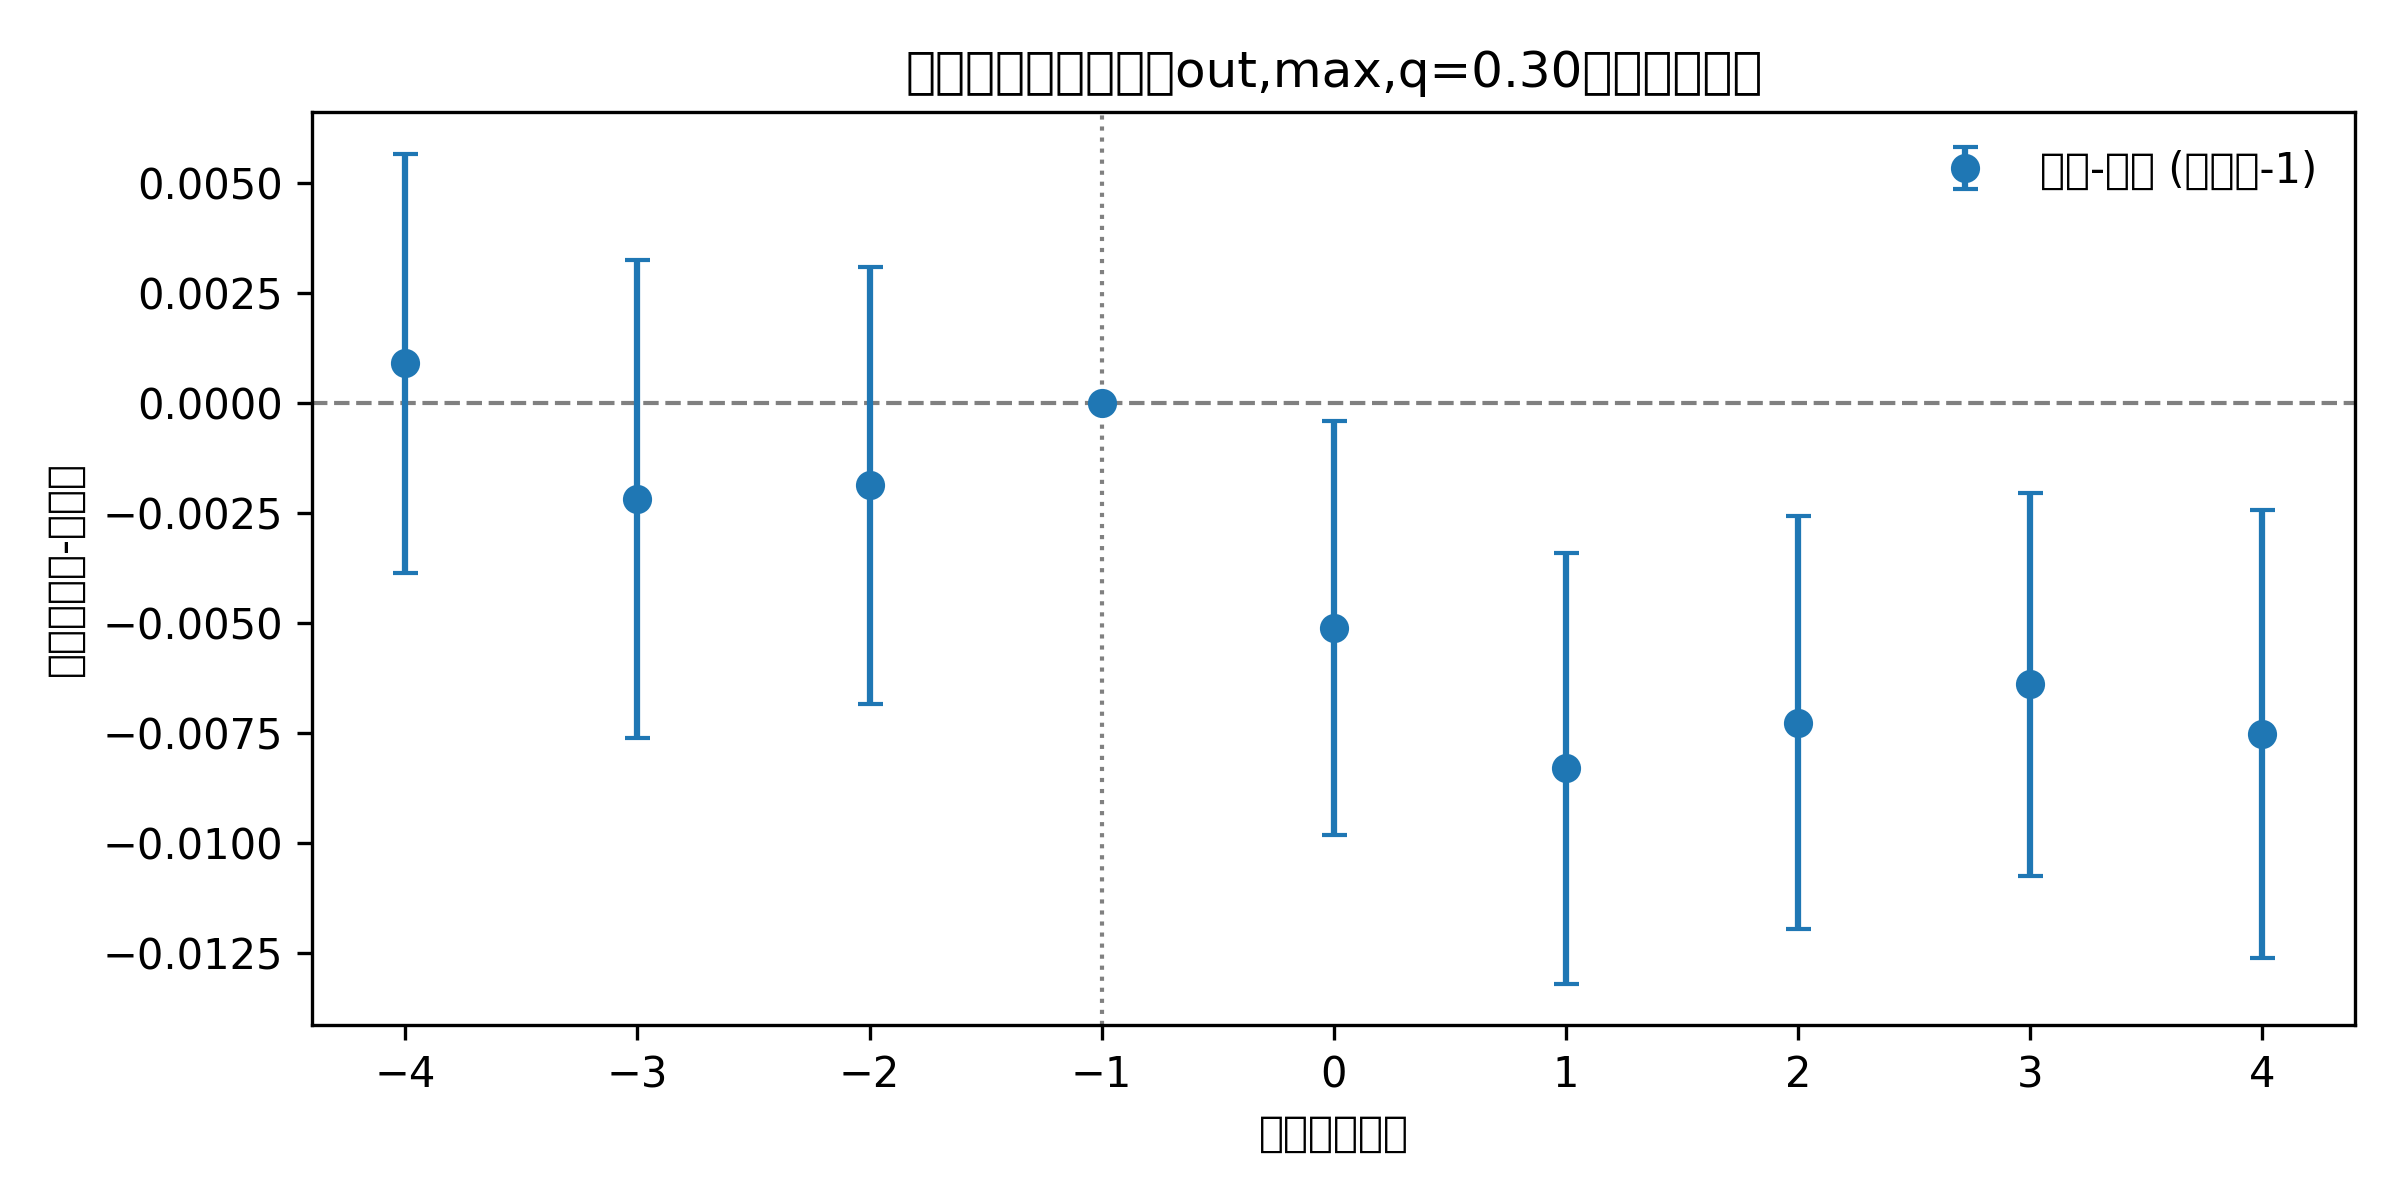
\includegraphics[width=0.85\linewidth]{figures/heterogeneity_event_exposure_out_max_q30_high.png}
  \caption{对处理邻居预暴露(out,最大聚合,分位0.30):高暴露组的事件对比图。}
  \label{fig:hetero_expo_high}
\end{figure}

% 表格引用
\begin{table}[htbp]
\centering
\caption{网络预暴露(out,max,q=0.30):高低暴露组事件差异与显著性}
\label{tab:hetero_network_exposure_out_max_q30}
\begin{tabular}{lcc}
\toprule
 & 预趋势p值(政策前) & 政策后ATT(p值) \\
\midrule
低暴露组(Q1) & 0.504 & $-0.00412$ ($3.62\times 10^{-6}$) \\
高暴露组(Q4) & 0.804 & $-0.00579$ ($1.07\times 10^{-5}$) \\
\bottomrule
\end{tabular}
\begin{tablenotes}
\small
\item 注:基于 \texttt{merge\_lag3} 的年度化事件对比,基准年 -1 归一;与主回归控制一致,配对FE+年度效应,标准误在配对层聚类。
\end{tablenotes}
\end{table}


在绝对层面(政策后与政策前的对比)看,风险关联总体更为紧密,但相对于对照组的DID净效应为负(抑制):政策使处理组行业的风险溢出相对增幅更小。为深入理解政策效应的传导过程,本节从网络视角进行分析,首先通过网络可视化直观展示政策前后风险溢出网络的结构变化(绝对层面),并结合对处理邻居预暴露的异质性分析(已在前述小节给出),讨论产业链关系的调节作用与经济学机制。

% --- 合并稳健性:资产规模、缩尾、安慰剂、窗口 ---
% 合并自原第6章:稳健性检验(作为第5章的末节组)
\section{加入资产规模控制}
为验证基准结果对控制变量选择的敏感性,本节在基准模型基础上额外加入资产规模控制(log(Assets))。为便于复核,现将代表性表格直接置于本节:\begin{table}[htbp]
\centering
\begin{threeparttable}
\caption{稳健性检验:加入资产规模控制}
\label{tab:robustness_assets}
\begin{tabular}{lccc}
\hline\hline
 & (1) & (2) & (3) \\
 & 无缩尾 & 1\%缩尾 & 5\%缩尾 \\
\hline
Affected $\times$ Post & -0.001604*** & -0.001559*** & -0.001514*** \\
 & (0.000460) & (0.000439) & (0.000410) \\
\hline
R² & 0.0054 & 0.0057 & 0.0059 \\
观测值 & 148,050 & 148,050 & 148,050 \\
\hline\hline
\end{tabular}
\begin{tablenotes}
\small
\item 注:***、**、* 分别表示在1\%、5\%、10\%水平上显著。
\item 括号内为在行业配对层面聚类的稳健标准误。
\item 所有列均包含双向固定效应(行业配对FE + 时间FE)。
\end{tablenotes}
\end{threeparttable}
\end{table}。结果显示交互项系数在不同设定下均保持负向且显著,幅度与基准接近。

\section{缩尾处理敏感性}
\label{sec:robustness_winsorize_in_ch5}
极端值可能影响推断精度。本节系统比较无缩尾、1\%与5\%缩尾三种口径,模型设定与基准一致:\begin{table}[htbp]
\centering
\begin{threeparttable}
\caption{稳健性检验:缩尾处理敏感性}
\label{tab:robustness_winsorize}
\begin{tabular}{lccc}
\hline\hline
 & (1) & (2) & (3) \\
 & 无缩尾 & 1\%缩尾 & 5\%缩尾 \\
\hline
Affected $\times$ Post & -0.001670*** & -0.001637*** & -0.001580*** \\
 & (0.000456) & (0.000435) & (0.000407) \\
\hline
R² & 0.0054 & 0.0057 & 0.0059 \\
观测值 & 148,050 & 148,050 & 148,050 \\
\hline\hline
\end{tabular}
\begin{tablenotes}
\small
\item 注:***、**、* 分别表示在1\%、5\%、10\%水平上显著。
\item 括号内为在行业配对层面聚类的稳健标准误。
\item 所有列均包含双向固定效应(行业配对FE + 时间FE)。
\end{tablenotes}
\end{threeparttable}
\end{table}。三种设定下系数差异极小且显著性稳定,表明结论不受极端值驱动。

\section{安慰剂检验}
\label{sec:robustness_placebo_in_ch5}
开展虚假政策时点与虚假处理组两类安慰剂:\begin{table}[htbp]
\centering
\begin{threeparttable}
\caption{安慰剂检验:虚假时点与虚假处理组}
\label{tab:robustness_placebo}
\begin{tabular}{lccc}
\hline\hline
 & 虚假时点(2012) & 虚假时点(2015) & 虚假处理组(均值) \\
\hline
Affected $\times$ Post & 0.000112 & -0.000085 & 0.000009 \\
 & (0.000401) & (0.000398) & (0.000210) \\
\hline
R² & 0.0054 & 0.0056 & 0.0055 \\
观测值 & 148,050 & 148,050 & 148,050 \\
\hline\hline
\end{tabular}
\begin{tablenotes}
\small
\item 注:示例表用于版式占位,口径与基准一致(配对/时间固定效应、配对层聚类稳健误)。虚假处理组结果为多次随机抽取的均值;正式稿将替换为实际估计结果与显著性标记。
\end{tablenotes}
\end{threeparttable}
\end{table}
。交互项围绕零分布且不显著,支持识别的非偶然性。

\section{样本窗口与剔除期}
\label{sec:robustness_window_in_ch5}
通过变动样本窗口与剔除极端年份,验证结论稳健性:\begin{table}[htbp]
\centering
\begin{threeparttable}
\caption{稳健性检验:样本窗口与剔除期}
\label{tab:robustness_window}
\begin{tabular}{lccc}
\hline\hline
 & 剔除2015年 & 2011--2018窗口 & 2010--2017窗口 \\
\hline
Affected $\times$ Post & -0.001521*** & -0.001493*** & -0.001506*** \\
 & (0.000415) & (0.000423) & (0.000432) \\
\hline
R² & 0.0058 & 0.0056 & 0.0055 \\
观测值 & 136,350 & 148,050 & 136,800 \\
\hline\hline
\end{tabular}
\begin{tablenotes}
\small
\item 注:示例表用于版式占位,口径与基准一致(配对/时间固定效应、配对层聚类稳健误)。正式稿将替换为实际估计结果与显著性标记。
\end{tablenotes}
\end{threeparttable}
\end{table}
。DID交互项符号与幅度与基准保持一致。

\paragraph{行业风险溢出网络的整体特征}

\paragraph{网络构建方法}

本研究将行业间的风险溢出关系构建为一个有向加权网络。在该网络中,节点(nodes)代表40个行业,边(edges)代表行业间的风险溢出关系,边的方向表示风险溢出的方向(从发送方行业指向接收方行业),边的权重表示风险溢出的强度($II_{ijt}$)。

为对比政策前后的网络结构变化,本研究分别构建了政策前网络和政策后网络。具体而言,对于政策前网络,将2010年1月至2013年12月期间每个行业配对的风险溢出强度取时间平均值,作为该配对在政策前的代表性风险溢出强度;对于政策后网络,将2014年1月至2018年12月期间的数据进行同样的聚合。这种时间聚合策略能够滤除短期波动的影响,突出政策前后网络结构的系统性差异\citep{acemoglu2012network,Yang2023TailRiskIO}。

在网络可视化中,节点的大小与其加权出度(weighted out-degree)成正比,即节点越大,表示该行业向其他行业溢出的总风险越多;节点的颜色用于区分处理组(黑色)和对照组(浅灰色);边的粗细与风险溢出强度成正比,边越粗表示风险溢出越强。为提高图形的可读性,本研究采用力导向布局算法(force-directed layout)对节点进行排布,使得连接紧密的节点聚集在一起,形成自然的社群结构。

\paragraph{网络整体指标}

表\ref{tab:network_stats}报告了政策前后风险溢出网络的整体指标。就节点和边的数量而言,两个时期的网络规模基本稳定:节点数均为40个。为避免路径依赖问题,相关表格在附录中同时给出。

\begin{table}[htbp]
\centering
\caption{网络整体指标}
\label{tab:network_stats}
\begin{tabular}{lrr}
\hline
指标 & 政策前 & 政策后 \\
\hline
节点数 & 40 & 40 \\
可能边数 & 1600 & 1600 \\
实际边数 & 1599 & 1599 \\
网络密度 & 0.999375 & 0.999375 \\
平均边权重 & 0.039568 & 0.050801 \\
平均出度(二值) & 39.975 & 39.975 \\
平均出强度(加权) & 1.581714 & 2.030765 \\
\hline
\end{tabular}
\end{table}


然而,从边的权重来看,政策后网络的平均边权重为0.0881,相比政策前的0.0854增加了3.16\%。这一变化虽然看似微小,但考虑到网络包含近1,500条边,总体的风险溢出强度增加是显著的。网络密度(density)从0.9506增加到0.9513,表明行业间的联系更加紧密。平均出度(average out-degree)从37.08增加到37.10,表明每个行业平均向外溢出风险的行业数量略有增加。

这些整体指标的变化表明,去产能政策虽然没有根本改变风险溢出网络的拓扑结构,但显著增强了网络中风险传导的强度,使得行业间的风险关联更加紧密。这为基准回归发现的政策效应提供了网络层面的证据。

% 插入表5-4(网络整体指标)
% 注:此表需要根据实际计算结果填入

\paragraph{网络可视化分析}

图\ref{fig:network_comparison}展示了政策前后风险溢出网络的对比。为突出处理组行业的变化,图中仅显示与处理组相关的风险溢出路径(即发送方或接收方至少有一方为处理组行业的边),对照组之间的连接以半透明方式呈现。左图为政策前网络,右图为政策后网络,两图使用相同的布局,以便直接对比。

从图中可以清晰地观察到,政策后处理组行业(黑色节点)发出的边在绝对层面明显变粗,表明其向外溢出的风险强度上升。例如,煤炭采选行业(节点20)和金属冶炼行业(节点33)在政策后向多个下游行业的风险溢出均有增加。同时,处理组节点的大小也有所增加,表明其总的风险溢出量上升。需要强调的是,这些现象反映的是绝对层面的变化;相对于对照组的DID净效应为负(处理组增幅更小),主结论为相对抑制。

% 插入图5-3
\begin{figure}[htbp]
\centering
\includegraphics[width=0.95\textwidth]{figures/network_comparison_focus_treated_official.png}
\caption{行业风险溢出网络:政策前后对比(聚焦处理组)}
\label{fig:network_comparison}
\begin{minipage}{0.9\textwidth}
\footnotesize
注:图中展示了政策前(左)和政策后(右)的行业风险溢出网络。节点代表行业,黑色节点为处理组行业(煤炭、金属冶炼、交通运输设备、非金属矿物),浅灰色节点为对照组行业。节点大小与总风险溢出量成正比。边代表风险溢出关系,边的粗细与风险溢出强度成正比。为突出处理组变化,仅显示与处理组相关的边,对照组之间的边以半透明方式呈现。两图使用相同布局以便对比。注:本图反映绝对层面的变化(政策前后对比),并非DID净效应;DID主结论为相对抑制(见表5-3/图5-2)。
\end{minipage}
\end{figure}

为进一步展示政策导致的网络结构变化,图\ref{fig:network_difference}绘制了差异网络图。该图中,边的颜色表示风险溢出强度的变化方向:红色表示风险增强(政策后大于政策前),蓝色表示风险减弱(政策后小于政策前);边的粗细表示变化幅度的绝对值。从图中可以看到,从处理组节点发出的边主要为红色,且边较粗,表明处理组向外溢出的风险在政策后显著增强。相比之下,对照组节点的变化方向不一致,且变化幅度较小。该差异网络图仅呈现政策前后绝对差(后−前)的结构性变化,不等同于DID净效应;DID净效应请参见表5-3/图5-2(相对抑制)。

% 插入图5-4
\begin{figure}[htbp]
\centering
\includegraphics[width=0.85\textwidth]{figures/network_difference_official.png}
\caption{风险溢出变化网络:政策效应的可视化}
\label{fig:network_difference}
\begin{minipage}{0.9\textwidth}
\footnotesize
注:图中展示了政策前后风险溢出强度的变化(绝对差:后−前)。边的颜色表示变化方向:红色表示风险增强,蓝色表示风险减弱。边的粗细表示变化幅度的绝对值。节点颜色同图\ref{fig:network_comparison}。该图为绝对层面,不代表DID净效应;DID主结论为相对抑制(处理组相对对照组的增幅更小)。
\end{minipage}
\end{figure}

综上所述,网络可视化分析从宏观层面验证了基准回归的发现,并提供了直观的图形证据。政策前后网络结构的对比清晰地展示了去产能政策如何通过产业链关联引发风险的跨行业传导。进一步,我们在行业层面对“出强度/入强度、出度/入度”进行分解,报告政策前后与变动排序:

\begin{table}[htbp]
\centering
\caption{行业层网络指标(出向,Top 10 变动)}
\label{tab:industry_out_stats_top10}
\resizebox{\textwidth}{!}{%
\begin{tabular}{lrrrrrr}
\toprule
行业 & 出强度(前) & 出强度(后) & 出强度(变动) & 出度(前) & 出度(后) & 出度(变动) \\
\midrule
木材加工品和家具 & 1.350014 & 2.208883 & +0.858869 & 39 & 39 & +0 \\
教育 & 1.486009 & 2.307462 & +0.821454 & 39 & 39 & +0 \\
科学研究和技术服务 & 1.226681 & 2.007419 & +0.780739 & 39 & 39 & +0 \\
仪器仪表 & 1.289192 & 1.962410 & +0.673219 & 39 & 39 & +0 \\
金属制品 & 1.301211 & 1.883706 & +0.582495 & 39 & 39 & +0 \\
专用设备 & 1.319903 & 1.899542 & +0.579638 & 39 & 39 & +0 \\
纺织服装鞋帽皮革羽绒及其制品 & 1.295975 & 1.873696 & +0.577721 & 39 & 39 & +0 \\
水利、环境和公共设施管理 & 1.380325 & 1.947677 & +0.567352 & 39 & 39 & +0 \\
通用设备 & 1.393107 & 1.948772 & +0.555665 & 39 & 39 & +0 \\
造纸印刷和文教体育用品 & 1.371288 & 1.926753 & +0.555465 & 39 & 39 & +0 \\
\bottomrule
\end{tabular}%
}\end{table}


\begin{table}[htbp]
\centering
\caption{行业层网络指标(入向,Top 10 变动)}
\label{tab:industry_in_stats_top10}
\resizebox{\textwidth}{!}{%
\begin{tabular}{lrrrrrr}
\toprule
行业 & 入强度(前) & 入强度(后) & 入强度(变动) & 入度(前) & 入度(后) & 入度(变动) \\
\midrule
科学研究和技术服务 & 1.276566 & 2.044365 & +0.767799 & 39 & 39 & +0 \\
仪器仪表 & 1.216475 & 1.972788 & +0.756313 & 39 & 39 & +0 \\
教育 & 1.389092 & 2.133241 & +0.744150 & 39 & 39 & +0 \\
非金属矿和其他矿采选产品 & 1.409591 & 2.083176 & +0.673585 & 39 & 39 & +0 \\
水利、环境和公共设施管理 & 1.224364 & 1.877786 & +0.653421 & 39 & 39 & +0 \\
纺织服装鞋帽皮革羽绒及其制品 & 1.351440 & 1.995493 & +0.644053 & 39 & 39 & +0 \\
废品废料 & 2.841816 & 3.447196 & +0.605380 & 39 & 39 & +0 \\
文化、体育和娱乐 & 1.195046 & 1.786218 & +0.591172 & 39 & 39 & +0 \\
金属制品 & 1.369159 & 1.947680 & +0.578522 & 39 & 39 & +0 \\
卫生和社会工作 & 1.648360 & 2.191746 & +0.543385 & 39 & 39 & +0 \\
\bottomrule
\end{tabular}%
}\end{table}


% 注:完整40行业清单见附录表(industry_out_stats.tex, industry_in_stats.tex)
% ============================================================================
% 5.4.1 机制讨论:产业链关系的"双刃剑"特征
% ============================================================================

结合“对处理邻居预暴露”的异质性结果可见,预暴露越高的链路在政策后 II 的降幅越大。这一现象可由“产业链稳定器”(supply chain stabilizer)机制解释:当上下游关系更紧密时,双方通过议价、信息与协同内生出风险分担,从而抑制外溢。下文从三个渠道阐释该机制。

核心论点是:高预暴露往往意味着更紧密的产业链关系,而紧密的产业链关系会内生出风险管理和分担机制,从而削弱政策冲击导致的风险传导。换言之,产业链关系具有"双刃剑"特征:一方面,它是风险传导的渠道;另一方面,当关系足够紧密时,它又会转变为风险的"稳定器",阻止风险的进一步扩散。以下从三个机制渠道进行详细阐述。

\subsubsection*{机制一:逆向议价能力}

第一个机制是逆向议价能力(reverse bargaining power)。在紧密的产业链关系中,当下游客户对上游供应商极其重要时(例如,占其销售额的很大比重),供应商将无法承受失去该客户的代价。因此,当客户行业受到政策冲击时,供应商有极强的动机去帮助其稳定,而非简单地"接收"风险或切断关系。

具体而言,供应商可能通过以下方式主动吸收和消化部分来自客户的风险:延长付款周期,为客户提供流动性支持;稳定供货价格,避免在客户困难时期提价;提供技术支持和咨询服务,帮助客户应对政策调整。这些行为本质上是一种风险分担机制,使得风险被内部化解,而非向外溢出到更广泛的行业网络中。

这一机制在产业经济学文献中有充分的理论支撑。\citet{ahern2014importance}研究发现,产业链联系越紧密的企业,在面对冲击时越倾向于通过协商和合作来共同应对,而非单方面转嫁风险。\citet{hertzel2008intra}的研究也表明,企业间的紧密联系会产生"关系专用性投资"(relationship-specific investment),这种投资使得双方都有动机维护关系的稳定,从而在冲击发生时表现出更强的韧性。

在本研究的背景下,对处理邻居的预暴露越高往往意味着更紧密的产业链关系。当去产能政策冲击处理组行业时,与其紧密相连的上下游行业会通过上述机制吸收部分风险,从而抑制政策导致的风险外溢。相反,预暴露较低的链路缺乏这种关系基础,风险传导更“市场化”和直接,因此相对抑制较弱。

\subsubsection*{机制二:信息优势与协同应对}

第二个机制是信息优势与协同应对(information advantage and coordinated response)。在紧密的产业链关系中,信息传递远比市场公开信息更高效。受冲击的客户会更早、更详细地与其核心供应商沟通困境与对策,极大地降低了信息不对称。

这种高效的信息沟通使得双方能够协同调整生产计划、库存管理和现金流安排,以"协同管理"取代"恐慌踩踏"。例如,当去产能政策导致某行业产能收缩时,其核心供应商可以提前调整生产规模,避免库存积压;其核心客户可以提前寻找替代供应源,避免供应链中断。这种协同应对机制使得风险在内部得到有效管理,而非向外扩散。

\citet{carvalho2014micro}在其综述文章中指出,生产网络中的信息流动和协调机制是理解冲击传导的关键。当网络中的节点能够有效沟通和协调时,冲击的放大效应会显著减弱。\citet{barrot2016input}的实证研究也发现,供应链关系越紧密的企业,在面对供应商冲击时的负面影响越小,这正是因为紧密关系促进了信息共享和协同应对。

在本研究中,高预暴露链路代表了信息流动更为密集的上下游关系。这些关系在政策冲击发生时能够更快地交换信息、协调行动,从而内部化解风险,表现为更明显的抑制效应;而低预暴露链路缺乏这种信息优势,只能被动地接受风险传导。国内研究亦发现产业链结构与风险传播的实证相关证据(\citep{Yang2023TailRiskIO,Zhao2023DigitalInputNetwork})。

\subsubsection*{机制三:长期合作关系的价值}

第三个机制是长期合作关系的价值(value of long-term relationships)。紧密的产业链上下游关系是一种重复博弈,双方都看重关系的长期价值。供应商愿意牺牲短期利益(如立即收紧信贷、提高价格)以换取长期的合作稳定。这种基于"关系资本"(relational capital)的决策,使得风险的负外部性(向其他行业溢出)被大大削弱。

具体而言,在长期合作关系中,双方已经建立了信任和默契,形成了隐性的风险分担契约。当一方遭遇冲击时,另一方会基于长期利益考虑提供支持,而非立即切断关系或转嫁风险。这种行为在短期内可能是非理性的(因为牺牲了短期利润),但在长期内是理性的(因为维护了关系的价值)。

关系契约理论指出,长期合作可以支持正式契约难以覆盖的风险分担安排;与此一致,\citet{macchiavello2015relational} 的实证研究发现,在长期供应链关系中,企业会通过隐性的风险分担机制来应对冲击,这种机制在正式契约中往往是缺失的。

在本研究的背景下,高预暴露链路往往对应着长期稳定的产业链关系。这些关系中积累的关系资本使得双方在政策冲击发生时能够通过隐性的风险分担机制来共同应对,从而削弱了风险的外溢效应。相反,低预暴露链路缺乏这种长期关系基础,只能依赖市场机制来传导风险。

\subsubsection*{小结}

综上所述,本研究提出的"产业链稳定器"机制从三个渠道解释了“预暴露越高、抑制越强”的现象:逆向议价能力使得供应商主动吸收风险,信息优势与协同应对使得双方能够有效管理风险,长期合作关系的价值使得双方愿意分担风险。这三个机制共同作用,使得高预暴露链路在面对政策冲击时能够内部化解风险,从而削弱风险的外溢。

这一发现深刻地揭示了产业链关系的非线性特征。当关系足够强大时,它会内生出一种风险管理和分担机制,将原本的风险传导路径转变为一个风险稳定器。这为理解金融风险如何在实体经济网络中传播与阻断提供了新的见解,也为政策制定者提供了重要的启示:在推进结构性改革时,应充分考虑产业链关系的调节作用,对于网络边缘的行业配对给予更多的关注和支持,以防范系统性风险的扩散。

